\chapter{الفرميونات، ومصفوفات ديراك، وبحر ديراك}

بحر ديراك هو وجهتنا، لكن الطريق إليه مهم. قبل مواجهة الطاقة السالبة في النظرية النسبية للإلكترون، نحتاج إلى أداتين. أولًا يأتي جبر المؤثرات الذي يميز الفرميونات عن البوزونات. ثم تأتي مراجعة لمعادلة ديراك أحادية البعد، حيث يمكن رؤية كل توسيع للدالة الموجية من غير هندسة الأبعاد المكانية الثلاثة. وما إن يكتمل هذان العنصران حتى تفرض المعادلة ثلاثية الأبعاد بنيتها المصفوفية الخاصة، ويعود النقاش الافتتاحي عن حالات الفرميونات المملوءة والفارغة بوصفه المفتاح إلى البوزيترونات.

نستخدم \(c=\hbar=1\). ويدل الرمز الكبير \(P\) على مؤثر الزخم، ويدل الرمز الصغير \(p\) على قيمة ذاتية للزخم، وتدل الرموز الغليظة على نظائرهما ثلاثية الأبعاد.

\section{يتحول التبادل إلى جبر المؤثرات}

لننظر في جسيمين متماثلين، أحدهما عند \(x\) والآخر عند \(y\). ويدل الرمزان \(x\) و\(y\) على موضعين كاملين؛ وليسا إحداثيين ديكارتيين لجسيم واحد. وعند التأثير بمؤثري إنشاء على حالة الفراغ نحصل على
\begin{equation}
\lvert x,y\rangle
=
\psi^\dagger(x)\psi^\dagger(y)\lvert0\rangle.
\label{eq:l10-two-particle-state}
\end{equation}

في حالة البوزونات، يترك تبديل الخانتين الحالة من دون تغير:
\begin{equation}
\lvert x,y\rangle=\lvert y,x\rangle.
\end{equation}
وعلاقة المؤثرات التي تضمن هذا التناظر هي
\begin{equation}
\psi^\dagger(x)\psi^\dagger(y)
=
\psi^\dagger(y)\psi^\dagger(x).
\label{eq:l10-boson-exchange}
\end{equation}
مؤثرا الإنشاء البوزونيان متبادلان، لذا يمكننا عكس ترتيبهما من دون تغيير الحالة التي ينشئانها.

في حالة الفرميونات، يغير التبادل الإشارة:
\begin{equation}
\lvert x,y\rangle=-\lvert y,x\rangle.
\label{eq:l10-fermion-state-exchange}
\end{equation}
الإشارة الكلية لمتجه حالة معزول غير قابلة للرصد، لكن الإشارات النسبية بين البدائل قابلة للرصد، لذا يجب الاحتفاظ بإشارة السالب هذه باتساق. وتقتضي المعادلة~\eqref{eq:l10-fermion-state-exchange}
\begin{equation}
\psi^\dagger(x)\psi^\dagger(y)
=
-\,\psi^\dagger(y)\psi^\dagger(x).
\label{eq:l10-fermion-operator-exchange}
\end{equation}

\begin{figure}[htbp]
\centering
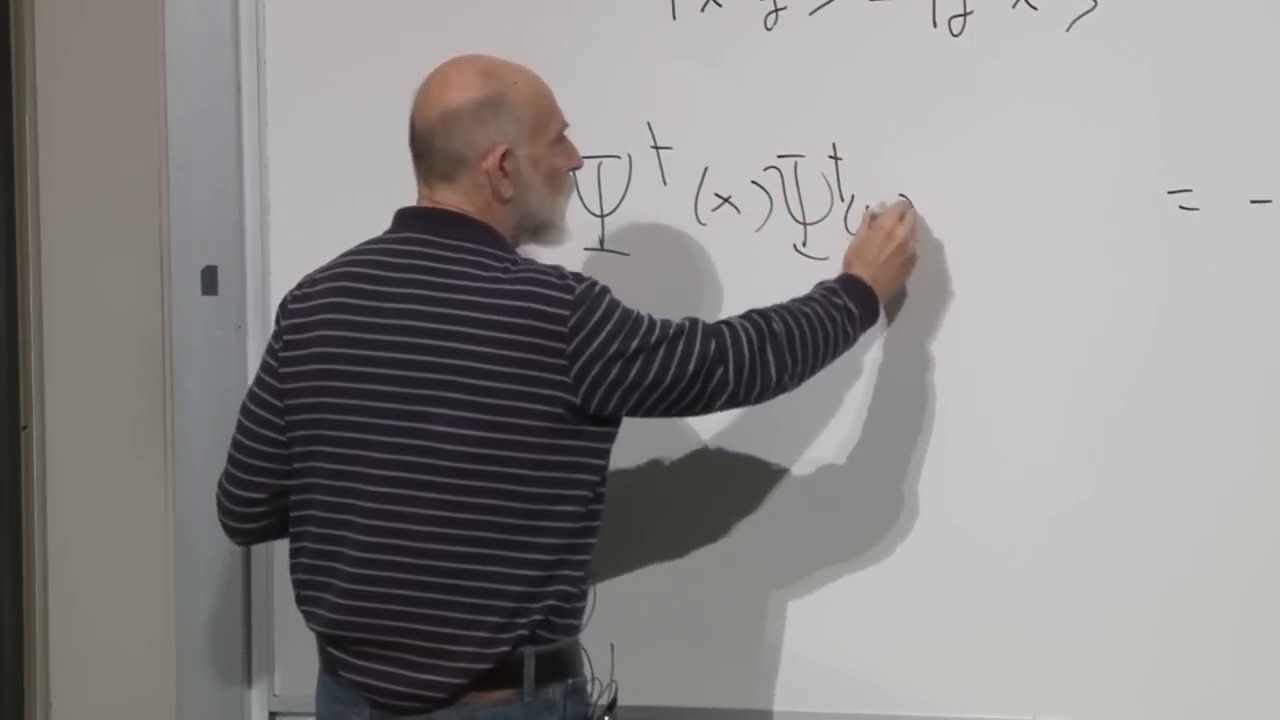
\includegraphics[width=0.94\linewidth]{lecture_10_figure_02.png}
\caption{العلاقة المكتوبة على اللوح التي تحقق التبادل الفرميوني. إن تبديل مؤثري الإنشاء يعكس إشارة حالة الجسيمين.}
\lectureframe{00:05:50}
\end{figure}

بالنسبة إلى أي مؤثرين \(A\) و\(B\)، نعرّف المبدلة المضادة بـ
\begin{equation}
\{A,B\}:=AB+BA.
\end{equation}
ولذلك تكون قاعدة التبادل
\begin{equation}
\{\psi^\dagger(x),\psi^\dagger(y)\}=0.
\label{eq:l10-creation-anticommutator}
\end{equation}
ويستبدل جبر الحقل الفرميوني المناظر المبدلات البوزونية بالمبدلات المضادة. ويجب التمييز بين استعمالين لهذه الكلمة: فمؤثرات الحقل تتبادل تبادلًا مضادًا بسبب إحصاء فيرمي، أما المصفوفات فستفعل ذلك لاحقًا من أجل إلغاء الحدود المتقاطعة في علاقة تشتت نسبية.

والآن ضع \(y=x\) في المعادلة~\eqref{eq:l10-creation-anticommutator}. ويصبح الضربان متماثلين:
\begin{align}
0
&=\{\psi^\dagger(x),\psi^\dagger(x)\}\\
&=2\,\psi^\dagger(x)\psi^\dagger(x).
\end{align}
ومن ثم
\begin{equation}
\bigl(\psi^\dagger(x)\bigr)^2=0.
\label{eq:l10-exclusion}
\end{equation}
إن محاولة إنشاء فرميونين متماثلين في حالة الجسيم الواحد نفسها تعطي متجه الصفر. وهذا هو مبدأ الاستبعاد في صيغة مؤثرية.

\begin{figure}[htbp]
\centering
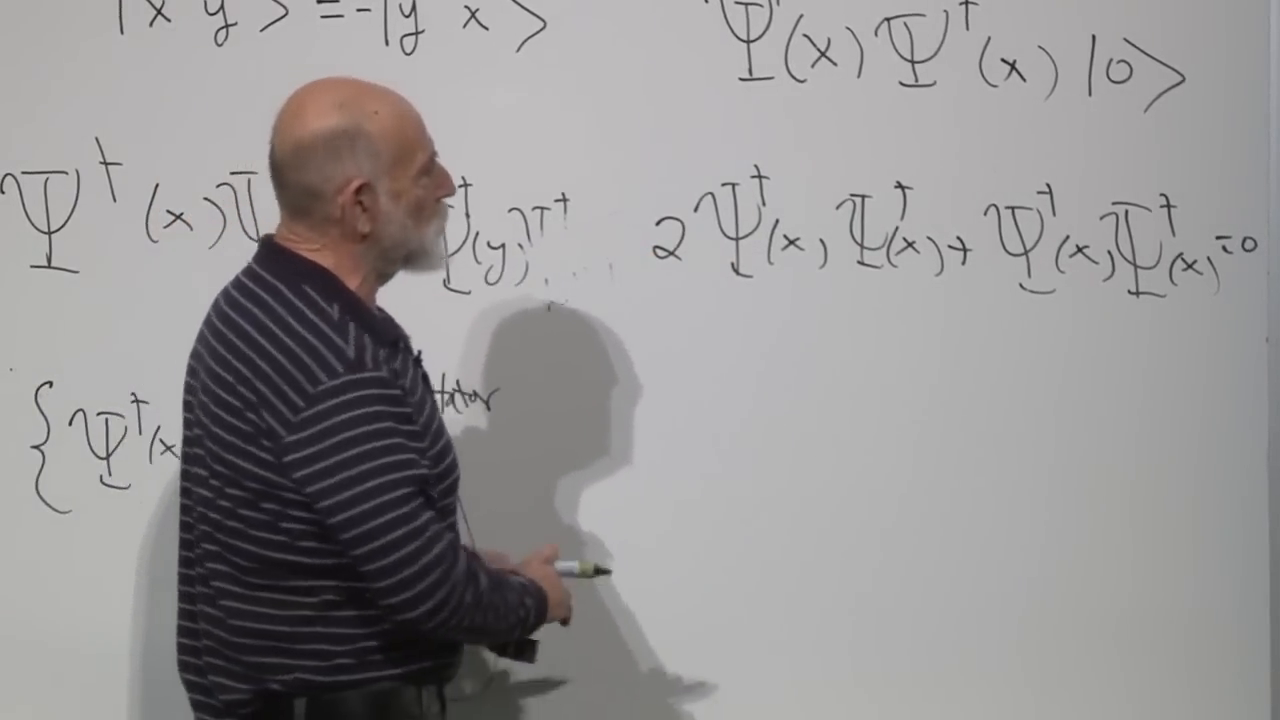
\includegraphics[width=0.94\linewidth]{lecture_10_figure_03.png}
\caption{التخصيص عند تساوي الحالتين على اللوح. يظهر حاصل ضرب مؤثر الخلق المكرَّر مرتين، ولذلك لا بد أن يساوي الصفر.}
\lectureframe{00:08:04}
\end{figure}

\begin{figure}[htbp]
\centering
\begin{adjustbox}{max width=\linewidth}
\begin{tikzpicture}[node distance=1.25cm,>=Latex]
\node[draw,rounded corners,align=center,inner sep=7pt] (a)
  {$\{\psi^\dagger(x),\psi^\dagger(x)\}=0$};
\node[draw,rounded corners,align=center,inner sep=7pt,right=of a] (b)
  {$2(\psi^\dagger(x))^2=0$};
\node[draw,rounded corners,align=center,inner sep=7pt,right=of b] (c)
  {$(\psi^\dagger(x))^2=0$};
\draw[->,thick] (a) -- (b);
\draw[->,thick] (b) -- (c);
\end{tikzpicture}
\end{adjustbox}
\caption{إعادة بناء حجة الاستبعاد من دون خطوات اللوح الوسيطة التي مُحيت جزئيًا.}
\end{figure}

\section{لماذا تكون حالتا الامتلاء والفراغ متناظرتين لفرميون}

ثمّة فرق ثانٍ بين المؤثرات البوزونية والفرميونية، وهو أدق من مبدأ الاستبعاد وجوهري لاحقًا. لنمط بوزوني واحد،
\begin{equation}
[a,a^\dagger]=1,
\qquad
n=0,1,2,\ldots.
\end{equation}
فإن تبديل \(a\) و\(a^\dagger\) يغيّر إشارة المبادل. وحتى لو لم يُسمَّ المؤثران إلا \(A\) و\(B\)، لأخبرتنا الجبرية أيُّ ترتيب يرفع عدد الإشغال وأيُّه يخفضه.

ولسُلَّم الإشغال البوزوني اتجاه أيضًا. فمؤثر الإبادة يبلغ في النهاية \(\lvert0\rangle\) ويعطي صفرًا، في حين يمكن لمؤثر الخلق أن يستمر إلى ما لا نهاية:
\begin{align}
a\lvert0\rangle&=0,\\
a^\dagger\lvert n\rangle&\propto\lvert n+1\rangle,
\qquad n=0,1,2,\ldots.
\end{align}
وقلب هذا السلم رأسًا على عقب لا يعيد إنتاج الطيف نفسه. فله قاع ولا قمة له.

ولنمط فرميوني واحد،
\begin{equation}
\{a,a^\dagger\}=1,
\qquad
a^2=(a^\dagger)^2=0,
\qquad
n=0,1.
\label{eq:l10-fermion-mode}
\end{equation}
ينقل مؤثر الخلق الحالة الفارغة إلى الحالة الممتلئة ثم يتوقف:
\begin{equation}
a^\dagger\lvert0\rangle=\lvert1\rangle,
\qquad
a^\dagger\lvert1\rangle=0.
\end{equation}
ويقوم مؤثر الإبادة بالعكس:
\begin{equation}
a\lvert1\rangle=\lvert0\rangle,
\qquad
a\lvert0\rangle=0.
\end{equation}
لا توجد إلا حالتان، لذا يكون المخطط متناظرًا تحت تبديل الحالة الممتلئة بالحالة الفارغة و\(a\) بـ\(a^\dagger\). وما يزال للمؤثرين معنيان فيزيائيان مختلفان، لكن جبريتهما لم تعد تميّز أحدهما بوصفه مؤثر خلق والآخر بوصفه مؤثر إبادة. وهذا التناظر الصوري هو بذرة إعادة تأويل الجسيم-الفجوة.

\begin{classroomqa}
\lecturetimestamp{00:13:54}
\audiencequestion{إذا كان \((a^\dagger)^2=0\)، أفهذا تناقض، أم إنه يستلزم أن \(a^\dagger=0\)؟}
\lecturerresponse{لا هذا ولا ذاك. يمكن لمؤثر غير صفري أن يكون له مربع منعدم. هنا يأخذ \(a^\dagger\) \(\lvert0\rangle\) إلى \(\lvert1\rangle\)، ولكن لا توجد حالة مسموح بها فوق \(\lvert1\rangle\)، لذلك فإن تطبيقه مرتين يعطي صفرًا. والاستدلال نفسه يعطينا \(a^2=0\).}
\end{classroomqa}

احتفظ بهذا التناظر بين الحالتين الممتلئة والفارغة جانبًا. فعندما يُزال إلكترون سالب الطاقة، ستُعاد تسمية مؤثر الإبادة بوصفه مؤثر خلق بوزيترون. وليست هذه الخطوة تغييرًا اعتباطيًا في الترميز؛ بل إنها تستخدم على وجه الدقة جبر الفرميون ذي الحالتين الذي أُرسي هنا.

\section{بناء ديراك أحادي البعد}

لنعد الآن إلى جسيم واحد في بعد مكاني واحد. أبسط معادلة موجية نسبية من الرتبة الأولى هي
\begin{equation}
i\partial_t\psi=-\,i\partial_x\psi.
\label{eq:l10-right-mover}
\end{equation}
ومع \(P=-i\partial_x\) تصبح
\begin{equation}
H=P.
\end{equation}
ولحالة ذاتية للزخم يكون \(E=p\)، وتكون سرعتها الزمرية
\begin{equation}
v_g=\frac{dE}{dp}=1.
\end{equation}
فالزخم الموجب أو السالب، ومن ثم الطاقة الموجبة أو السالبة، ما يزال يعطي موجة تتحرك كوحدة واحدة إلى اليمين. إشارة \(p\) تغيّر نمط الطور، لا اتجاه الانتشار.

يجب أن يكون الجسيم ذو الكتلة قادرًا على الحركة في أيٍّ من الاتجاهين. أدخل مركبةً ثانية تحقق
\begin{equation}
H\psi_1=P\psi_1,
\qquad
H\psi_2=-P\psi_2.
\label{eq:l10-two-directions}
\end{equation}
تتحرك المركبة الأولى إلى اليمين، والثانية إلى اليسار. ضعْهما في عمود،
\begin{equation}
\Psi=
\begin{pmatrix}
\psi_1\\
\psi_2
\end{pmatrix},
\end{equation}
وعرّف
\begin{equation}
\alpha=
\begin{pmatrix}
1&0\\
0&-1
\end{pmatrix}.
\end{equation}
فتصبح المعادلتان
\begin{equation}
H\Psi=\alpha P\Psi.
\label{eq:l10-massless-one-d}
\end{equation}
وثمن إدراج الاتجاهين معًا هو درجة حرية داخلية جديدة ثنائية القيمة.

الاتجاه وحده لا يولِّد كتلة. أدخل مصفوفةً ثانية،
\begin{equation}
\beta=
\begin{pmatrix}
0&1\\
1&0
\end{pmatrix},
\end{equation}
وجرِّب
\begin{equation}
H=\alpha P+\beta m.
\label{eq:l10-massive-one-d}
\end{equation}
وتحقق المصفوفتان
\begin{equation}
\alpha^2=\beta^2=\mathbb{1},
\qquad
\{\alpha,\beta\}=0.
\label{eq:l10-one-d-algebra}
\end{equation}
ويعطي تربيع الهاملتوني
\begin{align}
H^2
&=(\alpha P+\beta m)^2\\
&=\alpha^2P^2+\beta^2m^2
  +(\alpha\beta+\beta\alpha)Pm\\
&=P^2+m^2.
\label{eq:l10-one-d-dispersion}
\end{align}
ويزيل المُبدِّل المضاد في المعادلة ~\eqref{eq:l10-one-d-algebra} الحدَّ غير المرغوب فيه الخطي في كلٍّ من \(P\) و\(m\).

المصفوفة غير القطرية \(\beta\) تقرن المركبتين الاتجاهيتين. ومن المفيد أن نتصور حد الكتلة على أنه يمزج باستمرار بين السعات المتحركة إلى اليمين والمتحركة إلى اليسار. ولا ينبغي أخذ هذه الصورة على نحو حرفي بوصفها جسيمًا يرتد ذهابًا وإيابًا على مسار مجهري، لكنها تبيّن لماذا يمكن لحزمة موجية ذات كتلة أن يكون لها متوسط سرعة دون سرعة الضوء وأن تمتلك إطار سكون، في حين أن مركبة كيرالية معزولة عديمة الكتلة لا تستطيع ذلك.

\begin{classroomqa}
\lecturetimestamp{00:23:37}
\audiencequestion{هل توجد دلالة فيزيائية أعمق لإدخال كلتا المركبتين الاتجاهيتين؟}
\lecturerresponse{نعم، ولكنها تظهر بوضوح أكبر في ثلاثة أبعاد. في هذه المرحلة هما مجرد المركبتين اللازمتين لوصف الانتشار في اتجاهين متعاكسين وللسماح باقتران كتلي غير قطري. وتفسيرهما اللاحق هو اليدوية، أو الكيرالية.}
\end{classroomqa}

\section{تفرض الأبعاد الثلاثة مصفوفات باولي}

في ثلاثة أبعاد مكانية، يكون الزخم متجهًا. ولذلك فإن هاملتونيًا خطيًا في الزخم وقياسيًا تحت الدورانات يوحي بمتجه آخر، هذه المرة متجهًا مركباته مصفوفات:
\begin{equation}
H=\boldsymbol{\alpha}\cdot\mathbf P
=\alpha_xP_x+\alpha_yP_y+\alpha_zP_z.
\label{eq:l10-three-d-ansatz}
\end{equation}

\begin{figure}[htbp]
\centering
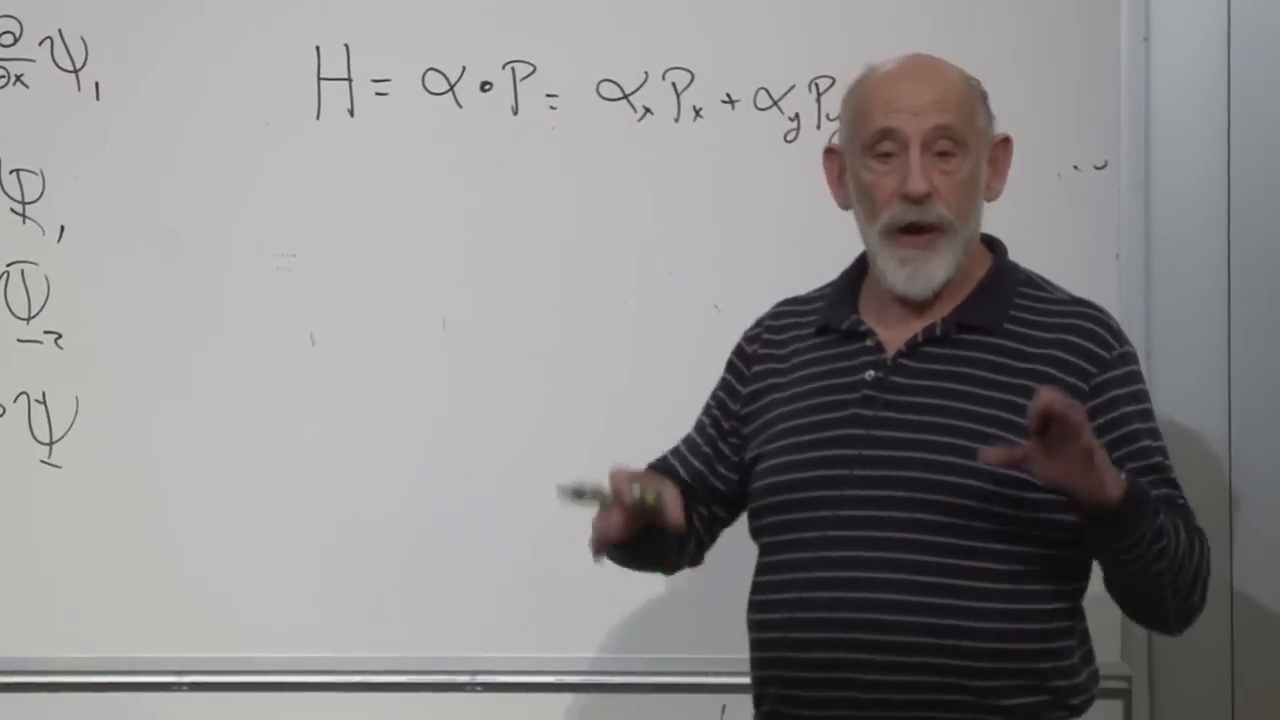
\includegraphics[width=0.94\linewidth]{lecture_10_figure_04.png}
\caption{الافتراض الابتدائي الثلاثي الأبعاد عديم الكتلة \(H=\boldsymbol{\alpha}\cdot\mathbf P\) عند النقطة التي تصبح فيها مصفوفة واحدة متجهًا مؤلفًا من ثلاث مصفوفات.}
\lectureframe{00:26:00}
\end{figure}

لنبدأ من جديد بالحالة عديمة الكتلة. نحتاج إلى
\begin{equation}
H^2=\mathbf P^2=P_x^2+P_y^2+P_z^2.
\end{equation}
وبتوسيع مربع المعادلة ~\eqref{eq:l10-three-d-ansatz}،
\begin{align}
H^2
&=\alpha_x^2P_x^2+\alpha_y^2P_y^2\\
&\quad+\alpha_z^2P_z^2\\
&\quad+\{\alpha_x,\alpha_y\}P_xP_y\\
&\quad+\{\alpha_x,\alpha_z\}P_xP_z\\
&\quad+\{\alpha_y,\alpha_z\}P_yP_z.
\end{align}
تكون الحدود القطرية صحيحة إذا تحقق
\begin{equation}
\alpha_x^2=\alpha_y^2=\alpha_z^2=\mathbb{1},
\end{equation}
وتختفي جميع الحدود المتصالبة إذا تحقق
\begin{equation}
\{\alpha_i,\alpha_j\}=0,
\qquad i\ne j.
\label{eq:l10-alpha-anticommutation}
\end{equation}

ثلاث مصفوفات مألوفة \(2\times2\) تحقق ذلك تمامًا:
\begin{equation}
\sigma_x=
\begin{pmatrix}
0&1\\
1&0
\end{pmatrix},
\quad
\sigma_y=
\begin{pmatrix}
0&-i\\
i&0
\end{pmatrix},
\quad
\sigma_z=
\begin{pmatrix}
1&0\\
0&-1
\end{pmatrix}.
\label{eq:l10-pauli-matrices}
\end{equation}
وعليه فإن أحد الحلول هو
\begin{equation}
\alpha_i=\sigma_i,
\qquad
H=\boldsymbol{\sigma}\cdot\mathbf P.
\label{eq:l10-weyl-hamiltonian}
\end{equation}

\begin{figure}[htbp]
\centering
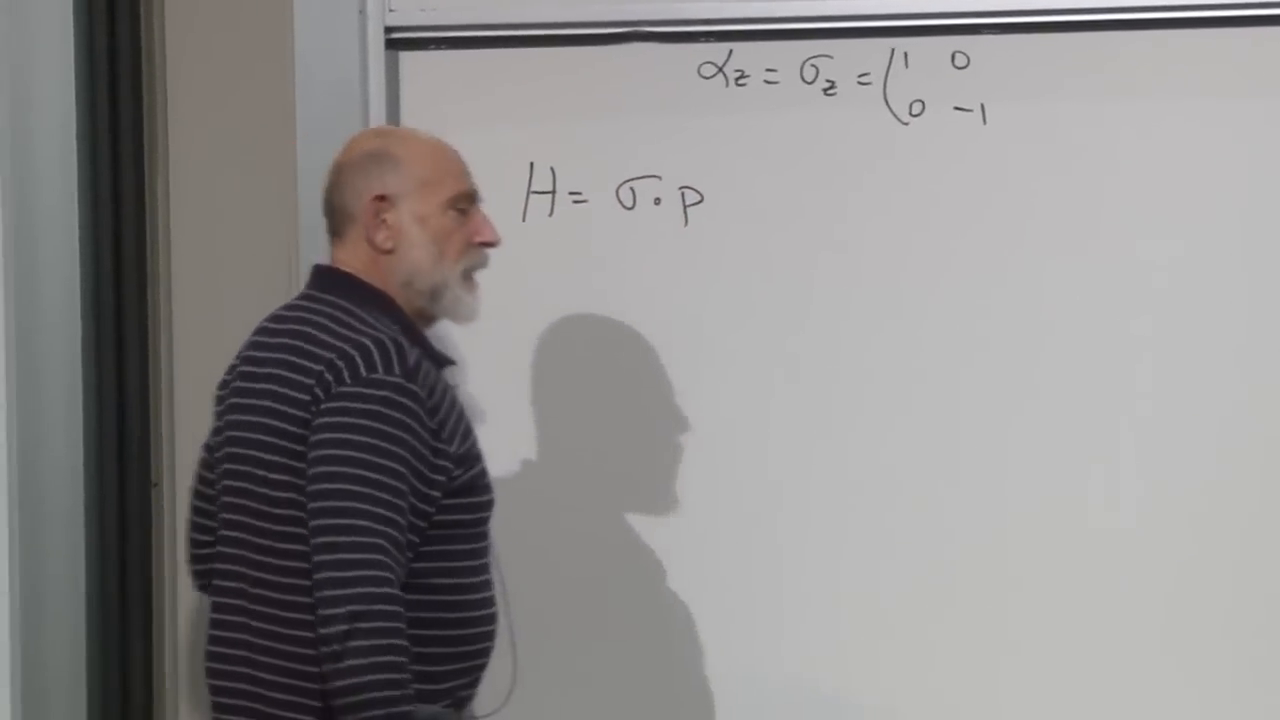
\includegraphics[width=0.94\linewidth]{lecture_10_figure_05.png}
\caption{الهاملتوني المدمج عديم الكتلة \(H=\boldsymbol{\sigma}\cdot\mathbf P\)، مع بقاء \(\alpha_z=\sigma_z\) ظاهرًا فوقه.}
\lectureframe{00:28:16}
\end{figure}

لحالة ذاتية للزخم،
\begin{equation}
\boldsymbol{\sigma}\cdot\mathbf p
=
|\mathbf p|\,\boldsymbol{\sigma}\cdot\widehat{\mathbf p}.
\end{equation}
للمؤثر \(\boldsymbol{\sigma}\cdot\widehat{\mathbf p}\) القيم الذاتية \(+1\) و\(-1\)، ولذلك
\begin{equation}
E=\pm|\mathbf p|.
\end{equation}
في هذه النظرية ذات المركبتين، تكون درجة الحرية الباولية في حالة الطاقة الموجبة مصطفةً مع الزخم، بينما تكون في حالة الطاقة السالبة مصطفةً بعكس اتجاهه. وهذا الاصطفاف مقيد؛ وليس اتجاهاً للّف المغزلي يمكن ضبطه على نحو مستقل عند تثبيت إشارة الطاقة.

\begin{classroomqa}
\lecturetimestamp{00:30:10}
\audiencequestion{هل ينبثق اللف المغزلي من معادلة ديراك، أم أُدخل فيها لأن من المعروف سلفاً أن للإلكترون عزماً مغناطيسياً؟}
\lecturerresponse{هنا تعني عبارة «ينبثق» «ينشأ كنتيجة»، لا «يختفي». كان الشرط الابتدائي أن يكون لدينا هاملتوني خطي في الزخم يكون مربعه \(\mathbf P^2\). ولا تستطيع الأعداد العادية أن تحقق الجبر المطلوب، لكن مصفوفات باولي تستطيع ذلك. ومن ثم فإن بنيتها ذات المركبتين تظهر مع عملية جعله خطيًا نفسها. وهذا لا يثبت أن كل جسيم يجب أن يملك لفًا مغزليًا؛ بل يقول إن الجسيمات التي تصفها هذه المعادلة من نوع ديراك تحمل درجة الحرية السبينورية المناظرة.}
\end{classroomqa}

هذه إحدى الدروس المركزية في هذا البناء. ليست المصفوفات تسميات زخرفية تُضاف بعد العثور على المعادلة النسبية. بل إن محاولة أخذ جذر تربيعي موضعي لعلاقة التشتت النسبية هي التي تولّدها.

\section{لماذا تتطلب الكتلة أربعة مركبات}

جرّب أن تكرر بناء الكتلة أحادي البعد من دون توسيع نظرية \(2\times2\):
\begin{equation}
H=\boldsymbol{\sigma}\cdot\mathbf P+\beta m.
\label{eq:l10-failed-mass}
\end{equation}
افترض \(\beta^2=\mathbb{1}\). يحتوي مربعه على الحدود المطلوبة \(\mathbf P^2+m^2\)، لكنه يحتوي أيضًا على
\begin{equation}
m\sum_i\{\sigma_i,\beta\}P_i.
\end{equation}
ولإزالة هذا الحد، يجب أن تحقق المصفوفة \(\beta\)
\begin{equation}
\{\sigma_x,\beta\}
=
\{\sigma_y,\beta\}
=
\{\sigma_z,\beta\}
=0.
\label{eq:l10-impossible-beta}
\end{equation}
ولا تحقق أي مصفوفة \(2\times2\) ذلك. فمصفوفة الهوية تتبادل مع مصفوفات باولي الثلاث كلها، وكل مصفوفة \(2\times2\) عديمة الأثر هي تركيب خطي من مصفوفات باولي. وأي تركيب من هذا القبيل يفشل في أن يكون مضادَّ التبادل مع المركبة الموازية له. ولا يملك جبر \(2\times2\) مصفوفةً رابعة مستقلة من النوع المطلوب.

العلاج هو توسيع السبينور. فأربع مصفوفات يكون كل منها مضادَّ التبادل مع الأخريات ومربعاتها هي مصفوفة الهوية تظهر لأول مرة في تمثيل عقدي \(4\times4\). ولم يُختر هذا الحجم المصفوفي لأن الزمكان ذو أربعة أبعاد؛ بل لأنه أصغر فضاء مصفوفي قادر على تحقيق الجبر المطلوب.

هناك تمثيلات مكافئة كثيرة. إن تغييرًا وحيديًا في أساس السبينور يغيّر عناصر جميع المصفوفات من دون أن يغيّر أي تنبؤ فيزيائي. وما يهم هو المجموعة المجرّدة من العلاقات
\begin{equation}
\{\alpha_i,\alpha_j\}=2\delta_{ij}\mathbb{1},
\qquad
\{\alpha_i,\beta\}=0,
\qquad
\beta^2=\mathbb{1}.
\label{eq:l10-dirac-algebra}
\end{equation}

\begin{classroomqa}
\lecturetimestamp{00:37:38}
\audiencequestion{هل يمكن اعتبار \(\beta\) مركبةً زمنيةً \(\alpha_t\)؟}
\lecturerresponse{ليس مباشرةً. فـ\(\alpha_i\) الثلاثة لا تتحد مع \(\beta\) بوصفها المكوّنات الأربعة لمتجه لورنتزي واحد. وبدلًا من ذلك، في الترميز المتغاير نعرّف \(\beta=\gamma^0\) و\(\alpha_i=\gamma^0\gamma^i\)؛ وتحقق مصفوفات \(\gamma^\mu\) الأربع جبر كليفورد للزمكان.}
\end{classroomqa}

أحد التمثيلات الكتلية الملائمة هو
\begin{equation}
\alpha_i=
\begin{pmatrix}
\sigma_i&0\\
0&-\sigma_i
\end{pmatrix},
\qquad
\beta=
\begin{pmatrix}
0&I_2\\
I_2&0
\end{pmatrix}.
\label{eq:l10-block-representation}
\end{equation}
تضمن مصفوفات باولي في الكتل القطرية أن تكون \(\alpha_i\) المختلفة مضادّةَ التبادل بعضها مع بعض. وتضمن كتل الهوية خارج القطر في \(\beta\) أن تكون \(\beta\) مضادّةَ التبادل مع كل \(\alpha_i\).

\begin{figure}[htbp]
\centering
\includegraphics[width=0.94\linewidth]{lecture_10_figure_06.png}
\caption{التمثيل الكتلي \(4\times4\) على السبورة. تسجّل المعادلات العليا المبدّلات المضادة المطلوبة؛ أما المصفوفات الكاملة فمصوغة في المعادلة ~\eqref{eq:l10-block-representation}.}
\lectureframe{00:41:10}
\end{figure}

هاملتوني الجسيم ذي الكتلة هو الآن
\begin{equation}
H=\boldsymbol{\alpha}\cdot\mathbf P+\beta m
=
\begin{pmatrix}
\boldsymbol{\sigma}\cdot\mathbf P&mI_2\\
mI_2&-\boldsymbol{\sigma}\cdot\mathbf P
\end{pmatrix}.
\label{eq:l10-massive-dirac}
\end{equation}
وباستخدام المعادلة ~\eqref{eq:l10-dirac-algebra}،
\begin{equation}
H^2=\mathbf P^2+m^2.
\end{equation}
ولذلك فالبنية ذات المركبات الأربعة ليست تزويقًا اختياريًا. إنها أصغر بنية تسمح بكل من الزخم ثلاثي الأبعاد وحد الكتلة مع إبقاء المعادلة من الرتبة الأولى.

\section{الكيرالية ومعنى المركبات الإضافية}

ما التمييز الفيزيائي الذي أضافه هذا التوسيع؟ ابدأ بالكتلة العلوية عديمة الكتلة،
\begin{equation}
H_R=\boldsymbol{\sigma}\cdot\mathbf P,
\end{equation}
وبالكتلة السفلية عديمة الكتلة،
\begin{equation}
H_L=-\boldsymbol{\sigma}\cdot\mathbf P.
\end{equation}
في حالات الطاقة الموجبة يكون في الأولى العزم المغزلي محاذيًا للزخم، وفي الثانية مضادَّ المحاذاة له. وهذه لولبيتان متعاكستان. وفي نظرية عديمة الكتلة تكون اللولبية ثابتة تحت تحولات لورنتز الصحيحة، لأنه لا يستطيع أي راصد أن يتجاوز جسيمًا ذا مسار ضوئي ويعكس زخمه مع إبقاء عزمه المغزلي من دون تغيير. ولذلك تصف الكتلتان قطاعين كيراليين متعاكسين.

\begin{classroomqa}
\lecturetimestamp{00:41:28}
\audiencequestion{في بعد واحد كانت هناك حاجة إلى درجة حرية ثنائية إضافية لإدخال الكتلة. فما التمييز الفيزيائي المناظر في ثلاثة أبعاد؟}
\lecturerresponse{إنها يدوية السبينور. فالكتلتان \(2\times2\) تحملان علاقتين متعاكستين بين العزم المغزلي والزخم. إحداهما يمينية والأخرى يسارية. ونظرية \(4\times4\) تحتويهما معًا.}
\end{classroomqa}

حد الكتلة في المعادلة ~\eqref{eq:l10-massive-dirac} خارج القطر. فهو يحوّل سعة الكتلة العلوية إلى الكتلة السفلية والعكس:
\begin{equation}
\beta m
\begin{pmatrix}
\Psi_R\\
\Psi_L
\end{pmatrix}
=
m
\begin{pmatrix}
\Psi_L\\
\Psi_R
\end{pmatrix}.
\end{equation}
ولذلك فالكتلة اقتران بين كيراليتين متعاكستين.

\begin{classroomqa}
\lecturetimestamp{00:43:58}
\audiencequestion{هل يستطيع جسيم عديم الكتلة أن يغيّر كيراليته؟}
\lecturerresponse{ليس في الهاملتوني الحر عديم الكتلة المعروض هنا. فالكتلتان منفصلتان عن بعضهما، لذا تبقى الحالة التي تبدأ يمينيةً أو يساريةً كذلك. وحد الكتلة خارج القطر هو بالضبط ما يخلط بينهما عندما \(m\ne0\).}
\end{classroomqa}

هذه اللغة دقيقة في التمثيل الكتلي، لكن لا ينبغي المضي بعيدًا جدًا في صورة جسيم ينقلب ميكانيكيًا بين سهمين. والقول الفيزيائي هو الاقتران المصفوفي في معادلة الموجة.

\begin{classroomqa}
\lecturetimestamp{00:44:50}
\audiencequestion{هل هذه المصفوفات مضمَّنة في الكواتيرنيونات؟}
\lecturerresponse{ترتبط مصفوفات باولي ارتباطًا وثيقًا بوحدات الكواتيرنيون: فالمصفوفات \(-i\sigma_i\) مربعاتها \(-\mathbb{1}\) وتتكثر وفق النمط الكواتيرنيوني، مع اختلاف اصطلاحات الاتجاه. وتتطلب مصفوفات ديراك الكاملة جبر كليفورد الأكبر، ولا تلزم صلة الكواتيرنيون للحجة التالية.}
\end{classroomqa}

\begin{classroomqa}
\lecturetimestamp{00:46:34}
\audiencequestion{إذا كان اللفّ المغزلي عزمًا زاويًا، فهل يوجد هنا حدّ طاقة منفصل مرتبط به؟}
\lecturerresponse{لا يُضاف أي حد مستقل لجسيم حر. فبنية السبينور تدخل بالفعل في الهاملتوني الحركي عبر المصفوفات. أما اقتران اللفّ المغزلي بمجال مغناطيسي خارجي فسيدخل حدود تفاعل إضافية، لكن تلك مسألة مختلفة.}
\end{classroomqa}

\section{مصفوفات ألفا هي السرعة، لا اللفّ المغزلي}

لكل \(\alpha_i\) قيمتان ذاتيتان تساويان \(+1\) وقيمتان ذاتيتان تساويان \(-1\). والمركبات المختلفة لا تتبادل، لذلك لا يمكن قياسها كلها بدقة في آن واحد. ولتحديد ما الذي تمثله إحدى المركبات، استخدم معادلة هايزنبرغ. بالنسبة إلى مؤثر \(L\) بلا اعتماد صريح على الزمن،
\begin{equation}
\dot L=i[H,L].
\label{eq:l10-heisenberg}
\end{equation}
ويُثبَّت اصطلاح الإشارة هنا بتطور Schr\"odinger \(e^{-iHt}\).

طبّق المعادلة ~\eqref{eq:l10-heisenberg} على مؤثر الموضع \(x\). تعمل المصفوفات على فهارس السبينور وتتبادل مع الموضع، بينما الوحيد الذي لا يتبادل مع \(x\) هو \(P_x\):
\begin{align}
\dot x
&=i[\boldsymbol{\alpha}\cdot\mathbf P+\beta m,x]\\
&=i\alpha_x[P_x,x]\\
&=\alpha_x,
\label{eq:l10-velocity}
\end{align}
لأن \([P_x,x]=-i\). ومن ثم فإن \(\alpha_x\) هو المركبة \(x\) من مؤثر السرعة؛ وبالمثل،
\begin{equation}
\dot{\mathbf x}=\boldsymbol{\alpha}.
\end{equation}

\begin{classroomqa}
\lecturetimestamp{00:51:50}
\audiencequestion{هل يعطي قياس مركبة من السرعة حقًا \(+1\) أو \(-1\) فقط؟}
\lecturerresponse{نعم، بالنسبة إلى المؤثر الآني \(\alpha_i\) بوحدات \(c=1\). ولا يلزم أن تكون الحالة العامة حالةً ذاتية، لذلك يمكن أن تقع قيمتها المتوقعة في أي موضع بين هاتين القيمتين. وللحزمة الموجية المتحركة بسلاسة سرعة متوسطة دون سرعة الضوء عندما يكون الجسيم ذا كتلة.}
\end{classroomqa}

السرعة غير محفوظة:
\begin{equation}
\dot\alpha_x=i[H,\alpha_x]\ne0.
\end{equation}
فالحدود التي تحتوي على \(\alpha_y\) و\(\alpha_z\) و\(\beta\) لا تتبادل مع \(\alpha_x\). وبناءً على ذلك، تُظهر الحالة التي تحتوي على مركبات من الطاقة الموجبة والسالبة معًا مساهمةً اهتزازية سريعة في موضعها. وهذا هو \emph{zitterbewegung}، أي حرفيًا الحركة الارتعاشية.

بعد أخذ متوسط على أزمنة طويلة مقارنةً بالاهتزاز السريع، تكون السرعة النسبية المتوقعة
\begin{equation}
\overline{\mathbf v}=\frac{\mathbf p}{E},
\end{equation}
وتُختزل إلى \(\mathbf p/m\) لإلكترون بطيء.

\begin{classroomqa}
\lecturetimestamp{00:54:40}
\audiencequestion{هل ينتهك اهتزاز إلكترون حر من دون قوة خارجية قانون نيوتن؟}
\lecturerresponse{لا. يحفظ تناظر الإزاحة الزخم، ومن ثم \(\dot{\mathbf P}=0\). ومؤثر السرعة في ديراك ليس ببساطة \(\mathbf P/m\)، ويمكن لجزئه الاهتزازي السريع أن يتغير مع بقاء الزخم ثابتًا. أما الحركة بعد المتوسط الزمني فتخضع لعلاقة الجسيم الحر المتوقعة.}
\end{classroomqa}

\begin{classroomqa}
\lecturetimestamp{00:55:22}
\audiencequestion{هل تكون السرعة دائمًا \(c\)؟}
\lecturerresponse{إن القياس الآني لأحد \(\alpha_i\) له قيم ذاتية \(\pm c\)، لكن الحزمة الموجية ذات الكتلة تكون عمومًا تراكبًا ولها قيمة متوقعة أقل من سرعة الضوء. ومتوسط سرعتها الجماعية هو \(\mathbf p/E\).}
\end{classroomqa}

\begin{classroomqa}
\lecturetimestamp{00:55:30}
\audiencequestion{هل يمكن تصوير الاهتزاز على أنه الكتلة تغيّر السرعة؟}
\lecturerresponse{لا. الكتلة معلمة ثابتة. وينشأ الاهتزاز من عدم تبادل مؤثري السرعة والهاملتوني، أو على نحو مكافئ من التداخل بين قطاعات الطاقة، لا من كتلة متقلبة.}
\end{classroomqa}

\begin{classroomqa}
\lecturetimestamp{00:56:22}
\audiencequestion{هل يمكن أن يجد قياس آني السرعة مشيرةً في اتجاه ما بينما تشير الحركة المتوسطة إلى اتجاه آخر؟}
\lecturerresponse{نعم. فمؤثر المركبة له قيمتان ذاتيتان محددتان تمامًا، بينما تستعيد القياسات المتكررة أو المتوسطات الزمنية الانجراف الأكثر سلاسة.}
\end{classroomqa}

ويجب أيضًا استخدام كلمة اللفّ المغزلي بحذر. إن \(\alpha_i\) تتحول كمركبات للسرعة، أي كمتجه عادي. أما مؤثر اللفّ المغزلي الحقيقي في هذا التمثيل فهو
\begin{equation}
\mathbf S=\frac12\boldsymbol{\Sigma},
\qquad
\Sigma_i=
\begin{pmatrix}
\sigma_i&0\\
0&\sigma_i
\end{pmatrix}.
\label{eq:l10-spin-operator}
\end{equation}
وهو يختلف عن \(\alpha_i\) في إشارة الكتلة السفلى. فالمصفوفات وثيقة الصلة، لكن السرعة واللفّ المغزلي ليسا المرصود نفسه.

\section{الطاقة السالبة والفراغ الأدنى طاقة}

مشكلة الطاقة السالبة موجودة أصلًا قبل كل هذه البنية المصفوفية. عُد إلى المتحرك نحو اليمين في بعد واحد،
\begin{equation}
H=P.
\end{equation}
وبما أن \(p\) يمتد على الخط الحقيقي كله، فإن \(E=p\) ليس له حد أدنى.

لا يمكن أن يعني الفراغ مجرد حالة بلا جسيمات. بل يجب أن يكون الحالة التي لا يمكن استخلاص أي طاقة إضافية منها. فإذا كانت حالة فارغة تتيح لنا إضافة جسيم ذي طاقة سالبة، فنخفض الطاقة، ثم نضيف آخر، ونستمر إلى ما لا نهاية، فإن تلك الحالة الفارغة ليست فراغًا مستقرًا.

يوفّر إحصاء فيرمي مخرجًا تاريخيًا. نضع إلكترونًا واحدًا في كل حالة ذات طاقة سالبة. وكل إلكترون مضاف يخفّض الطاقة الكلية، لكن مبدأ الاستبعاد لا يسمح إلا بإلكترون واحد في كل حالة أحادية الجسيم. وما إن تمتلئ كل الحالات ذات الطاقة السالبة، حتى لا يعود أي إلكترون إضافي قادرًا على الهبوط إلى ذلك القطاع. وقد اعتبر ديراك هذا الترتيب الممتلئ هو الفراغ.

وسيفشل البناء نفسه للبوزونات. إذ يمكن لعدد اعتباطي من البوزونات أن يشغل حالة واحدة، ولذا يمكن لنمط بوزوني ذي طاقة سالبة أن يمتص جسيمات بلا حد. إن القيد الفرميوني \(n=0,1\)، الذي قُدِّم في بداية المحاضرة، هو بالضبط ما يوقف هذا الانحدار.

\begin{figure}[htbp]
\centering
\includegraphics[width=0.94\linewidth]{lecture_10_figure_07.png}
\caption{الصورة التاريخية لبحر ديراك على اللوح: سُلَّم من مستويات الطاقة السالبة مملوء حتى الخط الفاصل، وحالات الطاقة الموجبة فوقه.}
\lectureframe{01:02:45}
\end{figure}

\begin{figure}[htbp]
\centering
\begin{adjustbox}{max width=\linewidth}
\begin{tikzpicture}[x=1.05cm,y=0.72cm,>=Latex]
\draw[->] (0,-4.8) -- (0,4.8) node[above] {$E$};
\draw[thick] (-2.9,0) -- (3.2,0) node[right] {$E=0$};
\foreach \y in {-4,-3.3,...,-0.5} {
  \draw (-2.3,\y) -- (2.3,\y);
  \foreach \x in {-1.8,-1.2,...,1.8} {
    \fill[blue!65!black] (\x,\y) circle (1.6pt);
  }
}
\foreach \y in {0.8,1.6,...,4.0} {
  \draw (-2.3,\y) -- (2.3,\y);
}
\draw[red,very thick] (0.6,-2.6) circle (5pt);
\draw[red,->,very thick] (0.6,-2.35) .. controls (1.4,-0.4) and (1.2,1.6) .. (1.5,2.4);
\fill[red] (1.5,2.4) circle (2.5pt);
\node[right,red] at (0.85,-2.6) {hole};
\node[right,red] at (1.7,2.4) {$e^-$};
\node[left] at (-2.5,-2.2) {filled negative-energy states};
\end{tikzpicture}
\end{adjustbox}
\caption{إعادة بناء واضحة لإثارة فوق بحر ممتلئ: إن ترقية إلكترون واحد من حالات الطاقة السالبة تترك ثقبًا موجب الطاقة.}
\end{figure}

إن صورة البحر ليست إلا لغة تاريخية لإعادة ترتيب صحيحة للمؤثرات. ولا ينبغي الخلط بين شحنتها وطاقتها اللانهائيتين على المعنى الحرفي وبين كميات قابلة للرصد مباشرة؛ فإعادة الصياغة الحديثة ستزيل الحاجة إلى تخيّل إلكترونات مادية تملأ الفضاء.

\section{الثقب هو البوزيترون}

ومع امتلاء جميع الحالات ذات الطاقة السالبة، يكون نوعان من الإثارة ممكنين. يمكننا أن نضيف إلكترونًا ذا طاقة موجبة فوق البحر. أو يمكننا أن نزيل إلكترونًا واحدًا ذا طاقة سالبة ونترك ثقبًا.

للثقب شحنة معاكسة لشحنة الإلكترون المفقود. إن إزالة شحنة \(-e\) تغيّر الشحنة بمقدار \(+e\). وله أيضًا طاقة إثارة موجبة. فإذا كان للإلكترون المُزال \(E_-<0\)، فإن الطاقة المقاسة بالنسبة إلى الفراغ الممتلئ تتغيّر كما يلي
\begin{equation}
E_{\mathrm{hole}}=-E_->0.
\end{equation}
الثقب إثارة ذات طاقة موجبة وشحنة موجبة: البوزيترون.

يمكن لفوتون أن يرقّي إلكترونًا من البحر إلى حالة ذات طاقة موجبة. وبالنسبة إلى الفراغ، تحتوي الحالة النهائية على إلكترون وبوزيترون. وفي مخطط مرتب زمنيًا، من المتعارف عليه أن يُرسم تدفق عدد الإلكترونات إلى أعلى على خط الإلكترون، وأن يُرسم خط البوزيترون بالسهم المعاكس. فالأسهم تتعقب تدفق عدد الفرميونات أو الشحنة؛ وليست متجهات سرعة كلاسيكية صغيرة.

\begin{classroomqa}
\lecturetimestamp{01:05:14}
\audiencequestion{هل تتطلب هذه الصورة أعدادًا متساوية من الإلكترونات والبوزيترونات؟}
\lecturerresponse{ليس بالنسبة إلى حالة اعتباطية. فالانطلاق من الفراغ وإنشاء زوج متعادل يعطي واحدًا من كلٍّ منهما، لكن قد تحتوي الحالة أصلًا على فائض من الإلكترونات أو فائض من البوزيترونات. ويقيِّد انحفاظ الشحنة التفاعلات؛ لكنه لا يقتضي أن تضم كل حالة مسموح بها أعدادًا متساوية منهما.}
\end{classroomqa}

لم يكن ديراك يعلم في البداية أن الثقب سيكون جسيمًا مماثلًا للإلكترون في الكتلة، ومعاكسًا له فقط في الشحنة وغيرها من الأعداد الكمومية الجمعية. وقد قادت المعادلة وبناء الثقب إلى ذلك التنبؤ قبل أن يُدرَج البوزيترون في قائمة الجسيمات المألوفة.

\section{حقل فرميوني واحد يحتوي على إلكترونات وبوزيترونات}

يُدخِل مؤثر الحقل الصورة التاريخية في الجبر الحديث. ولنُهمِل مؤقتًا مؤشرات السبينور، وعوامل التطبيع، والاعتماد على الزمن. ويمكن توسيع حقل أحادي البعد، على نحو تخطيطي، كما يلي
\begin{equation}
\psi(x)
\sim
\int_{-\infty}^{\infty}dp\,a(p)e^{ipx}.
\label{eq:l10-full-field-integral}
\end{equation}
وبالنسبة إلى علاقة التشتت للحركة نحو اليمين \(E=p\)، فإن \(p\) الموجب يدل على طاقة موجبة، و\(p\) السالب يدل على طاقة سالبة. قسِّم التكامل:
\begin{equation}
\psi(x)
\sim
\int_0^\infty dp\,a(p)e^{ipx}
+
\int_{-\infty}^0 dp\,a(p)e^{ipx}.
\end{equation}
وفي الحد الثاني خذ \(p=-q\)، مع \(q>0\)، وأعِد تأويل إفناء إلكترون ذي طاقة سالبة في حالة ممتلئة على أنه إنشاء بوزيترون:
\begin{equation}
b^\dagger(q):=a(-q).
\end{equation}
وعندئذٍ
\begin{equation}
\psi(x)
\sim
\int_0^\infty dp\,
\left[
a(p)e^{ipx}
+
b^\dagger(p)e^{-ipx}
\right].
\label{eq:l10-electron-positron-split}
\end{equation}
وتعتمد الإشارات الدقيقة لأطوار الموجة المستوية على الاصطلاح الزمكاني؛ أمّا المضمون الثابت فهو أن \(\psi\) يحتوي على مؤثر إفناء لإلكترون ومؤثر إنشاء لبوزيترون.

\begin{figure}[htbp]
\centering
\includegraphics[width=0.94\linewidth]{lecture_10_figure_08.png}
\caption{انقسم تكامل الحقل إلى قطاعي الطاقة الموجبة والطاقة السالبة. ويعيد السطر السفلي تسمية مؤثر الإلكترون ذي الطاقة السالبة بوصفه مؤثر إنشاء لبوزيترون.}
\lectureframe{01:11:35}
\end{figure}

هنا تتجلى فائدة تناظر الامتلاء والفراغ في المعادلة~\eqref{eq:l10-fermion-mode}. فبالنسبة إلى الفرميونات، تسمح جبرية المؤثرات بإعادة التسمية من دون تغيير بنية علاقات التبادل المضاد.

يأخذ تآثر كهرومغناطيسي تخطيطي الصورة
\begin{equation}
H_{\mathrm{int}}
\sim
\int dx\,\psi^\dagger(x)\psi(x)A(x),
\label{eq:l10-qed-schematic}
\end{equation}
حيث يدل \(A\) على حقل الفوتون. ولأن كل حقل فرميوني يشتمل على مركبتي الإلكترون والبوزيترون، فإن مؤثرًا موضعيًا واحدًا يتضمن عدة قنوات:
\begin{align}
e^-&\longrightarrow e^-+\gamma,\\
e^-+e^+&\longrightarrow\gamma,\\
\gamma&\longrightarrow e^-+e^+,
\end{align}
إلى جانب العمليات العكسية والمتصالبة المقابلة. ويحسم انحفاظ الطاقة والزخم أيَّ القنوات ممكنة حركيًا في بيئة معينة. فعلى سبيل المثال، لا يستطيع فوتون حقيقي منفرد في الفراغ أن يُنشئ زوجًا من دون مشارك آخر يمتص الارتداد، مع أن الرأس الموضعي موجود في التآثر.

\begin{figure}[htbp]
\centering
\includegraphics[width=0.94\linewidth]{lecture_10_figure_09.png}
\caption{تضع السبورة جنبًا إلى جنب إصدارَ إلكترونٍ فوتونًا، وفناءَ زوج، والتآثر التخطيطي \(\psi^\dagger\psi A\). وتولِّد اختيارات مختلفة من مؤثرات الحقل نفسها القنوات المختلفة.}
\lectureframe{01:13:30}
\end{figure}

ومن ثم فإن جداءً واحدًا مدمجًا للحقول ينظِّم كثيرًا من التفاعلات التي تبدو مختلفة ظاهريًا. وقد وضع فاينمان لاحقًا القواعد التخطيطية المنهجية لحساب السعات، لكن قدرًا كبيرًا من بنية المؤثرات ظاهر هنا بالفعل.

\section{لغة الفراغ الحديثة وتشبيه بحر فيرمي}

\begin{classroomqa}
\lecturetimestamp{01:14:20}
\audiencequestion{كيف يصف الفيزيائيون المعاصرون هذا من دون التعامل مع الفراغ على أنه بحر ديراك بالمعنى الحرفي؟}
\lecturerresponse{إنهم يجرون إعادة التفسير على مستوى المؤثرات مباشرةً. فيُعاد تسمية إفناء إلكترون ذي طاقة سالبة بأنه إنشاء بوزيترون ذي طاقة موجبة، ويُعرَّف الفراغ بأنه الحالة التي تفنيها جميع مؤثرات إفناء الإلكترونات والبوزيترونات. والصياغة الناتجة متناظرة بين الجسيمات والجسيمات المضادة ولا تحتاج إلى بحر مادي.}
\end{classroomqa}

يبقى البحر التاريخي مفيدًا لأن منطقه له نظير قريب في المادة المكثفة. ففي بلورة، يملأ عدد ثابت من الإلكترونات أدنى حالات الجسيم الواحد المتاحة حتى مستوى فيرمي. والحالة الأرضية الممتلئة ليست فارغة. ورفع إلكترون واحد إلى ما فوق ذلك المستوى يترك حالة غير مشغولة تحته. وبالنسبة إلى الخلفية الممتلئة، تحمل الفجوة طاقة إثارة موجبة ويمكن أن تتصرف كحامل شحنة موجبة.

ثمة فروق مهمة. ففجوة الحالة الصلبة توجد في وسط، وكتلتها الفعالة واستجابتها الشحنية تعتمدان على بنية النطاقات. أما البوزيترون فهو جسيم مضاد أولي في الحقل الكمومي النسبي. ومع ذلك، فإن جبر الجسيم-الفجوة المشترك يجعل هذا القياس قويًا.

\begin{classroomqa}
\lecturetimestamp{01:17:14}
\audiencequestion{هل تعاني نظرية كلاين--غوردون للبوزونات التهاوي نفسه إلى حالات طاقة سالبة؟}
\lecturerresponse{لا. فمجال كلاين--غوردون المركب، إذا كُمِّم على نحو صحيح، يُنظَّم إلى جسيمات وجسيمات مضادة ذات طاقة موجبة من دون ملء بحر بوزوني. وتختلف معادلته من الرتبة الثانية وبنيته الكانونية عن بناء هاملتوني ديراك، لذا فإن حجة البحر الفرميوني التاريخية لا تُنقَل إليه من دون تغيير.}
\end{classroomqa}

\begin{classroomqa}
\lecturetimestamp{01:17:30}
\audiencequestion{من أين يأتي اللف المغزلي الواحد للبوزونات؟}
\lecturerresponse{ليس من إجراء الخطيّة باستخدام مصفوفات باولي المستعمل هنا. فلحقول اللف المغزلي الواحد قانون تحول لورنتز الخاص بها ومعادلات مجالها الخاصة. والاشتقاق الحالي يفسر البنية السبينورية لفرميونات ديراك، لا جميع اللفات المغزلية الممكنة للجسيمات.}
\end{classroomqa}

\begin{classroomqa}
\lecturetimestamp{01:17:46}
\audiencequestion{لماذا كان إحصاء فيرمي أساسيًا لحل الطاقة السالبة؟}
\lecturerresponse{لأن مبدأ الاستبعاد يقيِّد كل حالة بإلكترون واحد. فمتى شُغلت جميع حالات الطاقة السالبة، لم يعد أي إلكترون آخر يستطيع الهبوط إليها. أما الإشغال البوزوني فليس له مثل هذا الحد، ولذلك فإن بحرًا بوزونيًا ذا طاقة سالبة بالمعنى الحرفي سيبقى بلا قاع.}
\end{classroomqa}

\begin{classroomqa}
\lecturetimestamp{01:20:02}
\audiencequestion{هل التمييز بين الإلكترون والبوزيترون مجرد درجة حرية ثنائية أخرى، مثل الشحنة؟}
\lecturerresponse{في عدّ الحالات، لمجال ديراك ذي الكتلة حالتا لف مغزلي للإلكترون وحالتا لف مغزلي للبوزيترون، لذا فإن استعمال وسمين ثنائيين وسيلة تذكّر مفيدة. لكن التمييز بين الجسيم والجسيم المضاد ليس بتًا كموميًا داخليًا لإلكترون واحد يمكن تدويره على نحو مستقل: فكل إلكترون شحنته \(-e\)، وكل بوزيترون شحنته \(+e\)، وينشأ هذا التمييز من قطاعي التردد الموجب والتردد السالب بعد التكميم.}
\end{classroomqa}

ويثير البحر اللانهائي سؤالًا أخيرًا.

\begin{classroomqa}
\lecturetimestamp{01:20:54}
\audiencequestion{هل سيولِّد بحر ديراك اللانهائي ثابتًا كونيًا لا نهائيًا؟}
\lecturerresponse{إنه يكشف مشكلة طاقة الفراغ. تُسهِم أنماط نقطة الصفر البوزونية بـ \(+\tfrac12\hbar\omega\)، بينما تُسهِم الأنماط الفرميونية بالإشارة المعاكسة. يمكن أن تحدث إلغاءات صورية عندما تتطابق الأطياف، لكن طيفَي الإلكترون والفوتون لا يتطابقان، ومن المتوقَّع بقاء باقٍ هائل. من دون جاذبية، يمكن طرح إزاحة ثابتة للهاملتوني لأن فروق الطاقة وحدها هي التي تهم. أمّا مع الجاذبية، فإن لطاقة الفراغ المطلقة أثرًا ثقاليًا، ولذلك يصبح هذا الطرح مشكلة فيزيائية لا مجرد ترتيب حسابي.}
\end{classroomqa}

أما العودة الأخيرة فإلى معنى الكتلة.

\begin{classroomqa}
\lecturetimestamp{01:22:56}
\audiencequestion{هل يمكننا أن نقول المزيد عن الكيفية التي تربط بها الكتلة بين المركبتين اليسارية واليمنية؟}
\lecturerresponse{الصياغة الدقيقة موجودة أصلًا في الهاملتوني: فالحد غير القطري \(m\beta\) يحوِّل إحدى الكتلتين الكيراليتين إلى الأخرى. وأي تصوير أكثر ميكانيكية لعملية التقليب المجهرية هذه اختياري، وهو حتمًا غير مكتمل.}
\end{classroomqa}